\documentclass[11pt]{article}
\usepackage{fullpage}
\usepackage{hyperref}
\usepackage{amssymb}
\newcommand{\R}{\mathbb{R}}

\newcommand{\tb}{\textbf}

\hypersetup{
    colorlinks,
    citecolor=black,
    filecolor=black,
    linkcolor=black,
    urlcolor=black
}
\urlstyle{urlcolor=blue}
\usepackage{graphicx}
\graphicspath{{./figures/}}
\usepackage{pgfplots}
\usepgfplotslibrary{fillbetween}
\usetikzlibrary{patterns}
\usepackage{amsmath}
\DeclareMathOperator{\arcsec}{arcsec}
\DeclareMathOperator{\arccot}{arccot}
\DeclareMathOperator{\arccsc}{arccsc}
\DeclareMathOperator{\DNE}{DNE}
\setcounter{tocdepth}{2}
\renewcommand{\contentsname}{Table of Contents}

\title{AP Calculus BC Reference}
\author{Sidharth Baskaran}

\pgfplotsset{compat=newest}
\begin{document}
\maketitle
\tableofcontents
\newpage

\section{Limits and Continuity}\label{sec:limits-and-continuity}
\subsection{Evaluating Limits}\label{subsec:evaluating-limits}

\begin{enumerate}
    \item To simply evaluate $\lim_{x\to{c}}f(x)$, 
    plug in $c$ such that $f(c)=L$, the value of the limit.

    \item If $f(c)=\frac{0}{0}$, factor numerator and denominator, then cancel terms.
    
    \[lim_{x\to{0}}\frac{x^4+x^2}{x^3+3x^2}=
        \lim_{x\to{0}}\frac{x^2+1}{x+3}=\frac{1}{3}\]

    \item If $f(c)=\frac{0}{0}$ and radicals are involved, 
    then rationalize using conjugate and resubstitute.
                  
    \[lim_{x\to{9}}\frac{\sqrt{x}-3}{x-9}\]

    \item For limits that approach $\pm{\infty}$, cancel everything but 
    greatest degree terms from numerator and denominator, then re-evaluate.
\end{enumerate}

Given the problem to find the value of constant $c$ as below, observe that
when the limit is indeterminate, it is in the form $\frac{0}{0}$.
This is because a limit with just denominator as $0$ does not exist, so 
the indeterminate form is required.

\begin{gather*}
    \lim_{x\to{2}}\frac{x^2+cx+c-10}{x^2-3x+2}\\
    x^2-3x+2\vert_{x=2}=0\Rightarrow \lim_{x\to{2}}\frac{x^2+cx+c-10}{x^2-3x+2}=\frac{0}{0}\\
    x^2+cx+c-10\vert_2=3c-6=0\\
    c=2\\
\end{gather*}

\subsection{Horizontal Asymptotes}\label{subsec:horizontal-asymptotes}

Take limit to $\pm \infty$ (end behavior).

\subsection{Squeeze Theorem}\label{subsec:squeeze-theorem}

Near $x=c$, let $g(x)\leq{f(x)}\leq{h(x)}\;\forall{x}$, if $\lim_{x\to{c}}g(x)=L$ and $\lim_{x\to{c}}h(x)=L$,
then $\lim_{x\to{c}}f(x)=L$ must be true.

\bigskip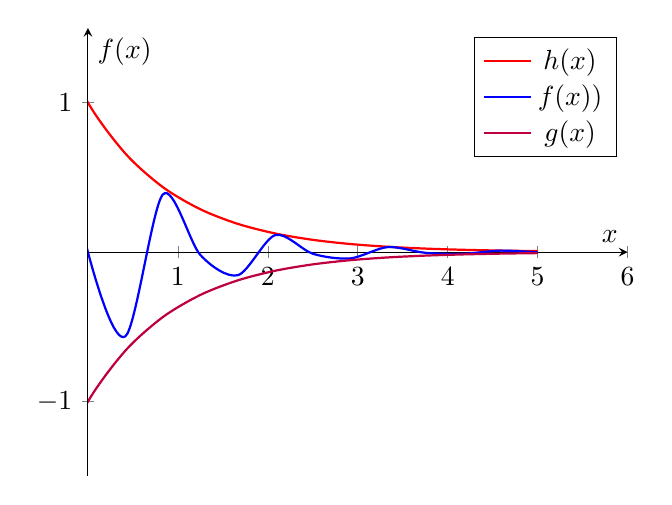
\begin{tikzpicture}
    \begin{axis}[
        xmin=0,xmax=6,
        ymin=-1.5,ymax=1.5,
        axis x line=middle,
        axis y line=middle,
        xlabel={$x$},
        ylabel={$f(x)$}
        ]
    \addplot[red,thick,smooth] {e^(-x)};
    \addlegendentry{$h(x)$}
    \addplot[blue,thick,smooth] {e^(-x)*sin(10*deg(x))};
    \addlegendentry{$f(x))$}
    \addplot[purple,thick,smooth] {-e^(-x)};
    \addlegendentry{$g(x)$}
    \end{axis}
\end{tikzpicture}

\subsection{Graphical Limits}\label{subsec:graphical-limits}

\begin{tikzpicture}
    \begin{axis}[
        xmin=-2,xmax=2,
        ymin=-2,ymax=3,
        axis x line=middle,
        axis y line=middle,
        axis line style=<->,
        xlabel={$x$},
        ylabel={$y$}
        ]
    \addplot[red,thick,domain=-1.5:1.5,<->] {x};
    \addplot[mark=*,fill=white] coordinates {(1,1)};
    \draw [dashed] (1,1) -- (1,0);
    \addlegendentry{$y=f(x)$}
    \end{axis}
\end{tikzpicture}\bigskip

Notice that the limit of $f(x)$ exists at $x=1$ though it is undefined at $(1,1)$.\\
Formally, $\lim_{x\to{1}}f(x)=1$ where $\lim_{x\to{1^-}}f(x)=\lim_{x\to{1^+}}f(x)$.

\subsection{Continuity}\label{subsec:continuity}

A function is continuous at an interior point if 
$\lim_{x\to{c}}f(x)=f(c)$.
It is continuous at a left endpoint if
$\lim_{x\to{a^+}}f(x)=f(a)$ and at a right endpoint if $\lim_{x\to{b^-}}f(x)=f(b)$.


\section{Derivatives}\label{sec:derivatives}
\subsection{Derivative Rules}\label{subsec:derivative-rules}

\begin{enumerate}
    \item Power Rule: $\frac{d}{dx}x^n=nx^{n-1}$
    \item Product Rule: $\frac{d}{dx}f(x)g(x)=f'(x)g(x)+g'(x)f(x)$
    \item Quotient Rule: $\frac{d}{dx}\frac{f(x)}{g(x)}=\frac{f'(x)g(x)-g'(x)f(x)}{(g(x))^2}$
    \item Chain Rule: $\frac{d}{dx}f(g(x))=g'(x)f'(g(x))$
    \item Logarithmic Derivatives
    \begin{enumerate}
        \item $\frac{d}{dx}\ln(f(x))=\frac{f'(x)}{f(x)}$
        \item $\frac{d}{dx}\log_{a}(f(x))=\frac{f'(x)}{\ln{a}f(x)}$
    \end{enumerate}
    \item Trigonometric Derivatives
    \begin{enumerate}
        \item $\frac{d}{dx}\sin{x}=\cos{x}$
        \item $\frac{d}{dx}\cos{x}=-\sin{x}$
        \item $\frac{d}{dx}\tan{x}=\sec^2{x}$
        \item $\frac{d}{dx}\cot{x}=-\csc^2{x}$
        \item $\frac{d}{dx}\sec{x}=\sec{x}\tan{x}$
        \item $\frac{d}{dx}\csc{x}=-\csc{x}\cot{x}$
    \end{enumerate}
    \item Inverse Trigonometric Derivatives
    \begin{enumerate}
        \item $\frac{d}{dx}\arcsin(f(x))=\frac{f'(x)}{\sqrt{1-(f(x))^2}}$
        \item $\frac{d}{dx}\arccos(f(x))=\frac{-f'(x)}{\sqrt{1-(f(x))^2}}$
        \item $\frac{d}{dx}\arctan(f(x))=\frac{f'(x)}{1+(f(x))^2}$
        \item $\frac{d}{dx}\arccot(f(x))=\frac{-f'(x)}{1+(f(x))^2}$
        \item $\frac{d}{dx}\arcsec(f(x))=\frac{f'(x)}{|f(x)|\sqrt{(f(x))^2-1}}$
        \item $\frac{d}{dx}\arccsc(f(x))=\frac{-f'(x)}{|f(x)|\sqrt{(f(x))^2-1}}$
    \end{enumerate}
\end{enumerate}

\subsubsection{Example of logarithmic differentiation}

\begin{center}
    Take $\ln$ of both sides, differentiate, then get in terms of $f'(x)$ and simplify.
\end{center}

\begin{gather*}
    f(x)=2^x\\
    \ln(f(x))=x\ln(2)\\
    \frac{f'(x)}{f(x)}=\ln{2}\\
    f'(x)=\ln{2}\cdot f(x)\\
    f'(x)=\ln{2}\cdot 2^x\\
\end{gather*}


\section{Applications of Derivatives}\label{sec:applications-of-derivatives}
\subsection{Implicit Differentiation}\label{subsec:implicit-differentiation}

\begin{center}
    Explained in the following example.
\end{center}

\begin{gather*}
    \frac{dy}{dx}(x^2+y^2+y=25)\\
    2x+2yy'+y'=0\\
    y'(2y+1)=-2x\\
    \frac{dy}{dx}=y'=\frac{-2x}{2y+1}\\
\end{gather*}

\subsection{Related Rates}

\subsubsection{Shadow Problem}

\begin{center}
    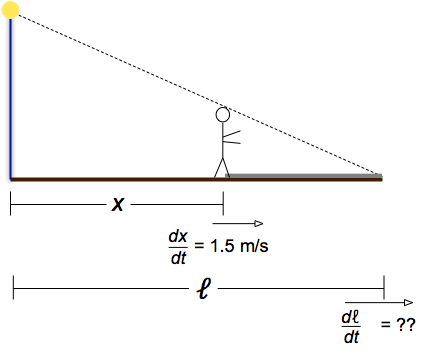
\includegraphics[scale=0.5]{rr_shadow_ov.png}
\end{center}

A 1.8-meter tall man walks away from a 6.0-meter lamp post at the rate of 1.5 m/s. 
The light at the top of the post casts a shadow in front of the man. 
How fast is the “head” of his shadow moving along the ground?

\vspace{5mm} 

Must find $\frac{dl}{dt}$. 
The strategy is to use similar triangles to relate $x$ and $l$.

\begin{center}
    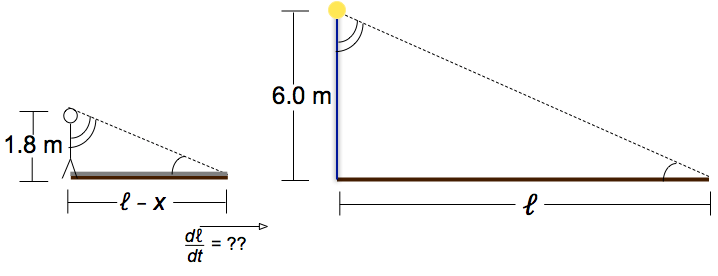
\includegraphics[scale=0.5]{rr_shadow_str.png}
\end{center}

\begin{gather*}
    \frac{l-x}{l}=\frac{1.8}{6.0}\\
    l-x=0.3l\\
    x-l=0.30l\\
    x=0.7l\\
\end{gather*}

\vspace{5mm}

\begin{gather*}
    0.7\frac{dl}{dt}=\frac{dx}{dt}\\
    \frac{dl}{dt}=\frac{1.5}{0.7}\\
    \frac{dl}{dt}=2.1 \frac{m}{s}\\
\end{gather*}

\subsubsection{Trough Problem}

\begin{center}
    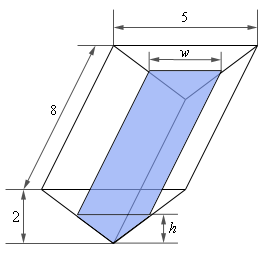
\includegraphics[scale=.5]{rr_trough.png}
\end{center}

A trough of water is 8 meters in length and its ends are in the shape of isosceles triangles whose width is 5 meters and height is 2 meters.
If water is being pumped in at a constant rate of 6 $m^3$/sec, 
at what rate is the height of the water changing when the water has a height of 120 cm? 
At what rate is the width of the water changing when the water has a height of 120cm?

\vspace{5mm}

It is known that $V'=6 m^3$/sec.
Need $h'$ when $h=1.2$.

\vspace{5mm}

The volume of the water in the tank is given by:

\begin{gather*}
    V=\frac{1}{2}base\times{height}\times{depth}\\
    =\frac{1}{2}hw(8)\\
    =4hw\\
\end{gather*}

Need to eliminate $w$ as target is $h'$.
Using similar triangles.

\begin{gather*}
    \frac{w}{5}=\frac{h}{2} \Rightarrow w=\frac{5h}{2} \Rightarrow V=10h^2\\
    V'=20hh' \Rightarrow 6=20(1.2)h' \Rightarrow h'=0.25m/sec\\
\end{gather*}

R.O.C of width can be found by manipulating similar triangles to get $V$ in terms of $w$ only.

\[h=\frac{2w}{5} \Rightarrow V=\frac{8w^2}{5}\]

Differentiate and substitute as before.

\subsection{L'Hopital's Rule}\label{subsec:l'hopital's-rule}

\subsubsection{Indeterminate Forms: $\frac{0}{0}$ or $\frac{\infty}{\infty}$}

\[\lim_{x\to{c}}\frac{f(x)}{g(x)}\]

Suppose that $f(x)=0$ and $g(x)=0$ and that $c \in \R$.

\[\lim_{x\to{c}}\frac{f(x)}{g(x)}=\lim_{x\to{c}}\frac{f'(x)}{g'(x)}\]

Process can be repeated.

\subsubsection{Indeterminate Forms: $\infty \cdot 0$ or $\infty - \infty$}

Requires that the limit be rewritten in fractional form for differentiation.

\begin{gather*}
    \lim_{x\to{0^+}}x\csc{x}\\
    x\csc{x}=\frac{x}{\sin{x}}\\
    \lim_{x\to{0}}\frac{x}{\sin{x}}=\frac{1}{\cos{x}}|_{0}=\frac{1}{1}=1\\
\end{gather*}

\subsubsection{Indeterminate Forms: $0^0$, $1^\infty$, or $\infty^0$}

Incorporates changes using logarithms in order to get limit in to the form
as shown before. 

\begin{gather*}
    L=\lim_{x\to{0^+}}x^x\\
    \ln{L}=x\ln{x} \Rightarrow -\infty \cdot 0\\
    \ln{L}=\lim_{x\to{0^+}}=\frac{\ln{x}}{\frac{1}{x}}=\frac{\frac{1}{x}}{\frac{-1}{x^2}}\\
    \ln{L}=\lim_{x\to{0^+}}-x=0\\
    e^{\ln{L}}=e^0\\
    L=1\\
\end{gather*}

Special example in the following form:

\[\lim_{x\to{c}}(d+\frac{a}{x})^{bx}=e^{ab}\]

\subsubsection{Limit Definition of Derivative}

In the form $f'(x)=\lim_{h\to{0}}\frac{f(x+h)-f(x)}{h}$, 
where the derivative is taken with respect to $h$.
By recognizing this form, the answer would be $\frac{d}{dx}f(x)$.

\section{Graphing and Analytical Applications}\label{sec:graphing-and-analytical-applications}
\subsection{Mean Value Theorem (MVT)}\label{subsec:mean-value-theoremnullmvtnull}

Given that $f(x)$ is continuous $\forall x \in [a,b]$ and differentiable
$\forall x \in (a,b)$, $\exists c \in (a,b)$ such that $f'(c)=\frac{f(b)-f(a)}{b-a}$.

\bigskip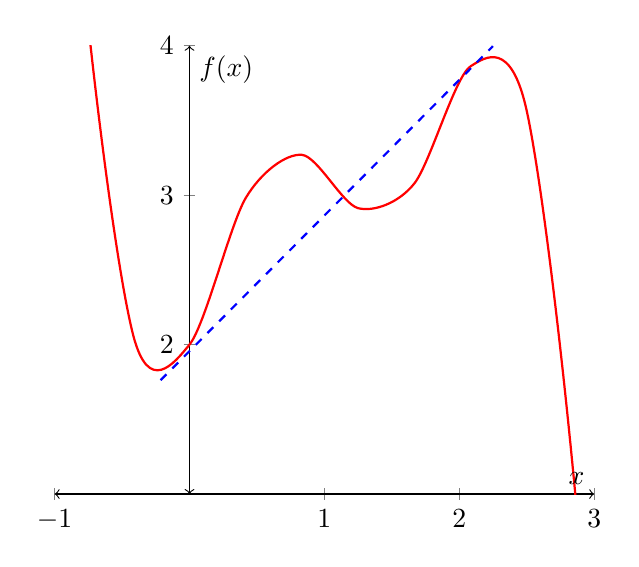
\begin{tikzpicture}
    \begin{axis}[
        xmin=-1,xmax=3,
        ymin=1,ymax=4,
        axis x line=middle,
        axis y line=middle,
        axis line style=<->,
        xlabel={$x$},
        ylabel={$f(x)$}
        ]
    \addplot[red,thick,smooth] {sin(3*deg(x))-x^3+3*x^2-x+2};
    \draw [dashed, thick, blue] (-.214,1.762) -- (2.249,3.997);
    \end{axis}
\end{tikzpicture}

\subsection{Intermediate Value Theorem (IVT)}\label{subsec:intermediate-value-theoremnullivtnull}

Let $f(x)$ be continuous $\forall x \in [a,b]$. Let $m$ between $f(a)$ and $f(b)$.
$\exists c \in (a,b)$ such that $f(c)=m$.

\bigskip\begin{tikzpicture}
    \begin{axis}[
        xmin=0,xmax=4,
        ymin=0,ymax=4,
        axis x line=middle,
        axis y line=middle,
        axis line style=<->,
        xlabel={$x$},
        ylabel={$f(x)$}
        ]
    \addplot[red,thick,smooth,domain=0:1] {x^2};
    \addplot[blue,thick,smooth,domain=1:1.5,dashed] {x^2};
    \addplot[red,thick,smooth,domain=1.5:5] {x^2};
    \node[label={180:{$a$}}] at (axis cs:1,1) {};
    \node[label={180:{$b$}}] at (axis cs:1.5,2.25) {};
    \end{axis}
\end{tikzpicture}

\subsection{Rolles' Theorem}\label{subsec:rolles'-theorem}

Given that $f(x)$ is continuous $\forall x \in [a,b]$ and differentiable
$\forall x \in (a,b)$ and $f(a)=f(b)$, then $\exists c \in (a,b)$ such that
$f'(c)=0$.

\subsection{Extreme Value Theorem (EVT)}\label{subsec:extreme-value-theoremnullevtnull}

If $f(x)$ is continuous $\forall x \in [a,b]$ then
$f(x)$ has a max and min value on $[a,b]$.

\bigskip\begin{tikzpicture}
    \begin{axis}[
        xmin=0,xmax=4,
        ymin=0,ymax=4,
        axis x line=middle,
        axis y line=middle,
        axis line style=<->,
        xlabel={$x$},
        ylabel={$f(x)$}
        ]
    \addplot[red,thick,smooth,domain=1:3] {x};
    \node[label={270:{$a$}}] at (axis cs:1,1) {};
    \node[label={90:{$b$}}] at (axis cs:3,3) {};
    \end{axis}
\end{tikzpicture}

\subsection{Fermat's theorem}\label{subsec:fermat's-theorem}

If $f(x)$ has a rel. max or min at $x=c$ and $f'(c)$ exists, then $f'(c)=0$.
However, there can be a rel. max/min when $f'(c)$ does not exist but implements
a sign change. 

\subsection{First Derivative Test for Local Extrema and Second Derivative Test}\label{subsec:first-derivative-test-for-local-extrema-and-second-derivative-test}

Determines where a function increases or decreases, which
denotes the maximums and mininums.
Is found from checking \emph{critical points}
where $f'(x)=0$.
Maximums and mininums occur where $f'(x)$ changes sign, 
which must be around a critical point.

\bigskip\begin{tikzpicture}
    \begin{axis}[
        xmin=0,xmax=7,
        ymin=-1.5,ymax=2.5,
        axis x line=middle,
        axis y line=middle,
        axis line style=<->,
        xlabel={$x$},
        ylabel={$f(x)$}
        ]
    \addplot[blue,thick,smooth,domain=0:2*pi] {sin(deg(x))};
    \node[label={90:{Max}}] at (axis cs:pi/2,1) {};
    \node[label={270:{Min}}] at (axis cs:3*pi/2,-1) {};
    \end{axis}
\end{tikzpicture}\bigskip

The second derivative test determines where the function
is \textbf{concave up} or \textbf{concave down}, or where
$f''(x)>0$ or $<0$ respectively.

\bigskip\begin{tikzpicture}
    \begin{axis}[
        xmin=0,xmax=7,
        ymin=-1.5,ymax=2.5,
        axis x line=middle,
        axis y line=middle,
        axis line style=<->,
        xlabel={$x$},
        ylabel={$f(x)$}
        ]
    \addplot[blue,thick,smooth,domain=0:2*pi] {sin(deg(x))};
    \node[label={90:{CCD}}] at (axis cs:pi/2,1) {};
    \node[label={270:{CCU}}] at (axis cs:3*pi/2,-1) {};
    \end{axis}
\end{tikzpicture}

\subsection{Second Derivative Test for Local Extrema}\label{subsec:second-derivative-test-for-local-extrema}

If $f'(x)$=0 and $f''(x)<0$, then $f(x)$ is the location of a local maxima.
Similarly if $f'(x)$=0 and $f''(x)>0$, then it is a local minima.
Can be visualized through a concave up/down image, where the apex of the curve
determines the extrema required.

\subsection{Absolute Maximums and Minimums (Candidates Test)}\label{subsec:absolute-maximums-and-minimumsnullcandidates-testnull}

Uses a chart like the following with $x$ values determined from endpoints and critical points of $f(x)$.

\bigskip
\begin{center}
    \begin{tabular}{|c|c|}
        \hline
        $x$ & $f(x)$\\
        \hline
        $a$ & $f(a)$\\
        \hline
        $x_1$ & $f(x_1)$\\
        \hline
        $x_2$ & $f(x_2)$\\
        \hline
        $b$ & $f(b)$\\
        \hline
    \end{tabular}
\end{center}

\subsection{Derivatives of Inverse Functions}\label{subsec:derivatives-of-inverse-functions}

Let $g(x)$ be $f^{-1}(x)$ and $(x,a)$ be the point.

\[g'(a)=\frac{1}{f'(g(a))}\]

\subsection{2D Particle Motion}\label{subsec:2d-particle-motion}

Fundamental equations are position, velocity, and acceleration.

\begin{gather*}
    x(t)\\
    v(t)=x'(t)\\
    a(t)=v'(t)=x''(t)\\
\end{gather*}

\subsubsection{Velocity}

A particle changes direction when $v(t)$ goes from $+$ to $-$.
The particle is moving to the left when $v(t)<0$ and to the right 
when $v(t)>0$.

\subsubsection{Speed}

Speed is denoted as $|v(t)|$.
A particle is speeding up when
$a(t)$ and $v(t)$ have the same sign and slowing down when they have
different signs.

\subsubsection{Find Next Position and Min/Max}

Uses FTC.

\[x(t_f)=x(t_i)+\int_{t_i}^{t_f}v(t)dt\]

Min/max problems are formatted as farthest to left or right.
Uses the candidates test for abs. max/min.
Use FTC to find position values. $t$-values are where $v(t)=0$.

\bigskip

Farthest to left $\Rightarrow$ abs. min., for right $\Rightarrow$ abs. max.

\subsubsection{Distance and Displacement}

Distance ($d$) is total distance traveled, ignores a change in direction,
displacement ($D$) accounts for this.

\begin{gather*}
    d=\int_{a}^{b}|v(t)|dt\\
    D=\int_{a}^{b}v(t)dt\\
\end{gather*}

\subsubsection{Average Speed and Velocity}

Average speed ($S$) is related to distance.
Average velocity ($V$) accounts for displacement.

\begin{gather*}
    S=\frac{\int_{a}^{b}|v(t)|dt}{b-a}\\
    V=\frac{\int_{a}^{b}v(t)dt}{b-a}\\
\end{gather*}

\subsection{Differentiability and Continuity}\label{subsec:differentiability-and-continuity}

A function is not neccesarily differentiable if it is continuous, but if it 
is differentiable, then it must be continuous.
Types of non-differentiable
points include corner points, cusps, and vertical tangents.

\subsubsection{Corner Points}

\[\lim_{x\to{c}}\frac{f(x)-f(c)}{x-c}=\DNE\]

\subsubsection{Vertical Tangents}

\[\lim_{x\to{c}}\frac{f(x)-f(c)}{x-c}=\pm \infty\]

\subsubsection{Cusps}

\begin{gather*}
    \lim_{x\to{c^+}}\frac{f(x)-f(c)}{x-c}=\pm \infty\\
    \lim_{x\to{c^-}}\frac{f(x)-f(c)}{x-c}=\mp \infty\\
\end{gather*}

\section{Integration}\label{sec:integration}
\subsection{Basic Rules}\label{subsec:basic-rules}

\begin{enumerate}
    \item FTC: $F(b)=F(a)+\int_{a}^{b}f(x)dx$
    \item Power rule: $\int{x^n}dx=\frac{x^{n+1}}{n+1}$
\end{enumerate}

\subsubsection{U-Substitution}

\begin{gather*}
    \int_{2}^{5}x(3x^2)dx \Rightarrow u=3x^2, du=6xdx\\
    \Rightarrow \frac{1}{6}\int_{12}^{75}udu\\
    \frac{1}{6}[\frac{u^2}{2}|_{75}-\frac{u^2}{2}|_{12}]\\
\end{gather*}

\subsubsection{Integration by Partial Fractions}

Factor denominator, separate into partial fractions, then integrate.

\begin{gather*}
    \int{\frac{1}{x^2-4}}dx \Rightarrow \frac{1}{x^2-4}=\frac{1}{(x+2)(x-2)}\\
    \frac{1}{(x+2)(x-2)} \Rightarrow \frac{A}{x+2}+\frac{B}{x-2} \Rightarrow A=-\frac{1}{4}, B=\frac{1}{4}\\
    \int{\frac{-\frac{1}{4}}{x+2}+\frac{\frac{1}{4}}{x-2}}dx=-\frac{1}{4}\ln{|x+2|}+\frac{1}{4}\ln{|x-2|}+C\\
\end{gather*}

\subsubsection{Trigonometric Integrals}

Trigonometric Integrals
\begin{itemize}
    \item $\int{\sin{x}}\:dx=-\cos{x}+C$
    \item $\int{\cos{x}}\:dx=\sin{x}+C$
    \item $\int{\tan{x}}\:dx=-\ln{\cos{x}}+C$
    \item $\int{\cot{x}}\:dx=\ln{\sin{x}}+C$
    \item $\int{\sec{x}}\:dx=\ln{(\sec{x}+\tan{x})}+C$
    \item $\int{\csc{x}}\:dx=\ln{(\csc{x}-\cot{x})}+C$
    \item $\int{\sec{x}\tan{x}}\:dx=\sec{x}+C$
    \item $\int{-\csc{x}\cot{x}}\:dx=\csc{x}+C$
    \item $\int{\sec^2{x}}\:dx=\tan{x}+C$
    \item $\int{-\csc^2{x}}\:dx=\cot{x}+C$
\end{itemize}
Inverse Trigonometric Integrals
\begin{itemize}
    \item $\int{\frac{dx}{f(x)^2+a^2}}=\frac{1}{a}\arctan{\frac{f(x)}{a}}+C$
    \item $\int{\frac{dx}{\sqrt{a^2-f(x)^2}}}=\arcsin{\frac{f(x)}{a}}+C$
\end{itemize}

\subsection{Properties of Integrals}\label{subsec:properties-of-integrals}

\begin{enumerate}
    \item $\int_{a}^{a}f(x)dx=0$
    \item If $f(x)$ is odd, $\int_{-a}^{a}f(x)dx=0$
    \item If $f(x)$ is even and $\int_{0}^{a}f(x)dx=k$, then $\int_{-a}^{a}f(x)dx=2k$
    \item $\int_{a}^{b}f(x)dx+\int_{b}^{c}f(x)dx=\int_{a}^{c}f(x)dx$
    \item If $\int_{a}^{b}f(x)dx=k$, then $\int_{b}^{a}f(x)dx=-k$
    \item If $f(x) \leq g(x)$ $\forall x \in [a,b]$ then $\int_{a}^{b}f(x)dx \leq \int_{a}^{b}g(x)dx$
    \item $\vert \int_{a}^{b}f(x)dx \vert \leq \int_{a}^{b}|f(x)|dx$
\end{enumerate}

\subsection{Riemann Sums}\label{subsec:riemann-sums}

\subsubsection{Riemann Sum Notation and Definite Integrals}

\[\lim_{n\to{\infty}}\sum_{k=1}^{n}f(a+k\Delta{x})\Delta{x}\]

In $\Delta{x}=\frac{b-a}{n}$ (the subintervals), $b$ is the end limit of the integral which is the same as 
$a+n\Delta{x}$.
This can be used to solve for $b$ given $a$. $x$ can be represented
as $a+k\Delta{x}$.

\[\int_{a}^{b}f(x)dx=\lim_{n\to\infty}\sum_{k=1}^{n}f(a+\frac{k(b-a)}{n})\frac{b-a}{n}\]

\subsubsection{Basic Riemann Sums}

Left sum: $(x_R-x_L)f(x_L)$

\bigskip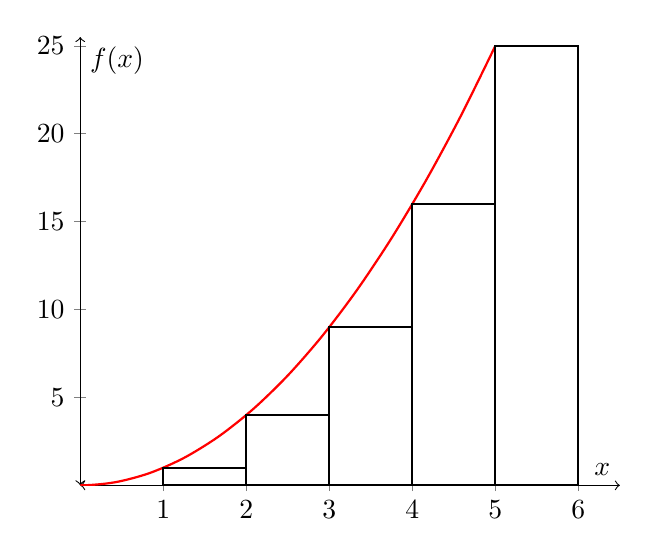
\begin{tikzpicture}
    \begin{axis}[
        xmin=0,xmax=6.5,
        ymin=0,ymax=25.5,
        axis x line=middle,
        axis y line=middle,
        axis line style=<->,
        xlabel={$x$},
        ylabel={$f(x)$}
        ]
    \addplot[red,thick,smooth] {x^2};
    \draw[draw=black,thick] (1,0) rectangle (2,1);
    \draw[draw=black,thick] (2,0) rectangle (3,4);
    \draw[draw=black,thick] (3,0) rectangle (4,9);
    \draw[draw=black,thick] (4,0) rectangle (5,16);
    \draw[draw=black,thick] (5,0) rectangle (6,25);
    \end{axis}
\end{tikzpicture}\bigskip

Right sum: $(x_R-x_L)f(x_R)$

\bigskip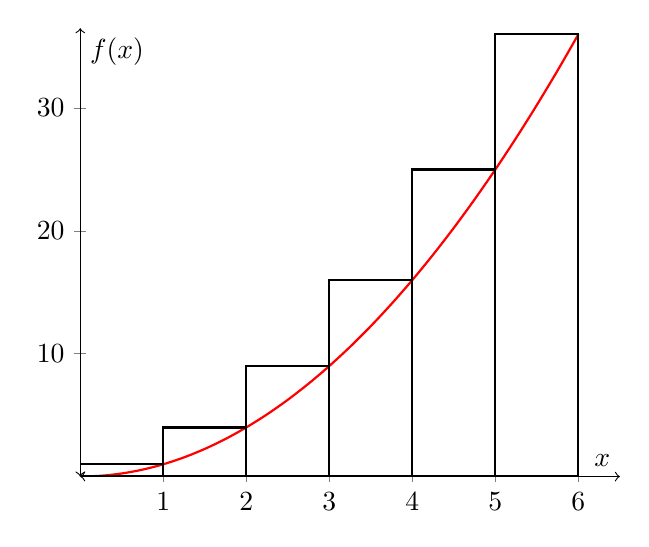
\begin{tikzpicture}
    \begin{axis}[
        xmin=0,xmax=6.5,
        ymin=0,ymax=36.5,
        axis x line=middle,
        axis y line=middle,
        axis line style=<->,
        xlabel={$x$},
        ylabel={$f(x)$}
        ]
    \addplot[red,thick,smooth,domain=0:6] {x^2};
    \draw[draw=black,thick] (0,0) rectangle (1,1);
    \draw[draw=black,thick] (1,0) rectangle (2,4);
    \draw[draw=black,thick] (2,0) rectangle (3,9);
    \draw[draw=black,thick] (3,0) rectangle (4,16);
    \draw[draw=black,thick] (4,0) rectangle (5,25);
    \draw[draw=black,thick] (5,0) rectangle (6,36);
    \end{axis}
\end{tikzpicture}\bigskip

Midpoint sum: $(x_R-x_L)f(x_L+\frac{x_R-x_L}{2})$

\bigskip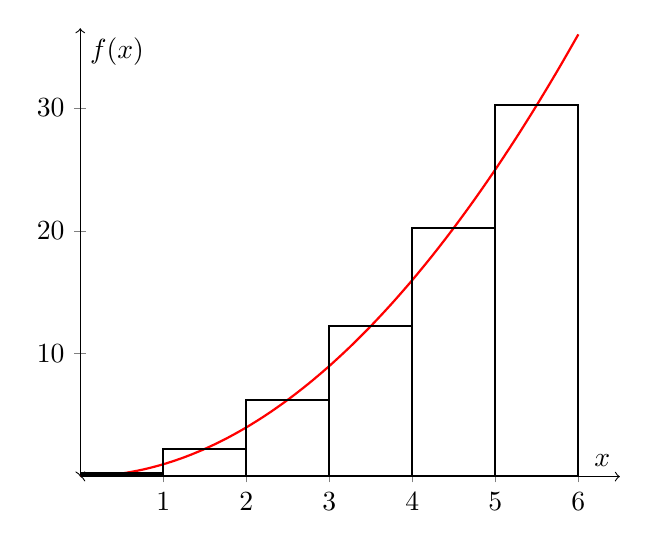
\begin{tikzpicture}
    \begin{axis}[
        xmin=0,xmax=6.5,
        ymin=0,ymax=36.5,
        axis x line=middle,
        axis y line=middle,
        axis line style=<->,
        xlabel={$x$},
        ylabel={$f(x)$}
        ]
    \addplot[red,thick,smooth,domain=0:6] {x^2};
    \draw[draw=black,thick] (0,0) rectangle (1,0.25);
    \draw[draw=black,thick] (1,0) rectangle (2,2.25);
    \draw[draw=black,thick] (2,0) rectangle (3,6.25);
    \draw[draw=black,thick] (3,0) rectangle (4,12.25);
    \draw[draw=black,thick] (4,0) rectangle (5,20.25);
    \draw[draw=black,thick] (5,0) rectangle (6,30.25);
    \end{axis}
\end{tikzpicture}\bigskip

Trapezoidal sum: $\frac{1}{2}(f(x_R)+f(x_L))(x_R-x_L)$

\bigskip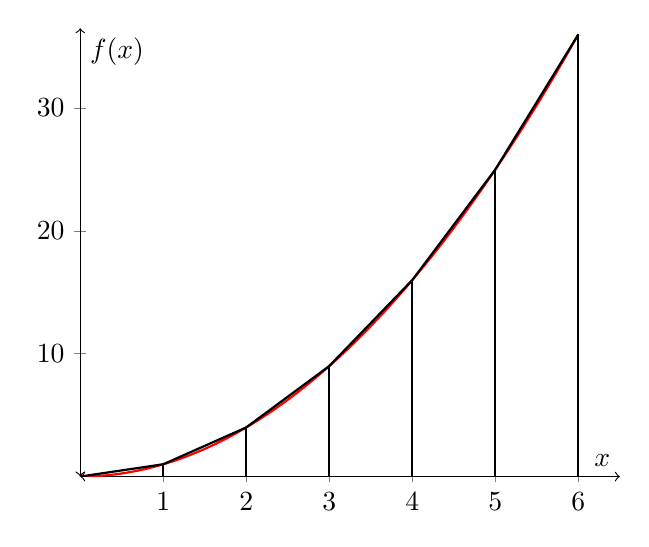
\begin{tikzpicture}
    \begin{axis}[
        xmin=0,xmax=6.5,
        ymin=0,ymax=36.5,
        axis x line=middle,
        axis y line=middle,
        axis line style=<->,
        xlabel={$x$},
        ylabel={$f(x)$}
        ]
    \addplot[red,thick,smooth,domain=0:6] {x^2};
    \draw[black,thick] (0,0)--(1,1);
    \draw[black,thick] (1,1)--(1,0);
    \draw[black,thick] (1,1)--(2,4);
    \draw[black,thick] (2,4)--(2,0);
    \draw[black,thick] (2,4)--(3,9);
    \draw[black,thick] (3,9)--(3,0);
    \draw[black,thick] (3,9)--(4,16);
    \draw[black,thick] (4,16)--(4,0);
    \draw[black,thick] (4,16)--(5,25);
    \draw[black,thick] (5,25)--(5,0);
    \draw[black,thick] (5,25)--(6,36);
    \draw[black,thick] (6,36)--(6,0);
    \end{axis}
\end{tikzpicture}

\subsection{Integration by Parts}\label{subsec:integration-by-parts}

\[\int{f'(x)g(x)}dx=f(x)g(x)-\int{g'(x)f(x)}dx\]

Choose $g(x)$ in order of \textbf{logs, inverse, algebraic, trig, exponential}.

\subsubsection{Example}

\begin{gather*}
    \int{x\sqrt{x+1}}dx \Rightarrow g(x)=x, f'(x)=\sqrt{x+1}\\
    =\frac{x}{2}(x+1)^{3/2}-\int{\frac{1}{2}(x+1)^{3/2}}dx\\
    =\frac{x}{2}(x+1)^{3/2}-\frac{1}{5}(x+1)^{5/2}+C\\
\end{gather*}

\subsubsection{Tabular Method}

Negate every second entry under derivative column.

\[\int{x^2\sin{x}}\:dx \Rightarrow f(x)=x^2,\;g(x)=\sin{x}\]

\begin{center}
    \begin{tabular}{|c|c|}
        \hline
        $f(x)$ & $g(x)$\\
        \hline
        $x^2$ & $\sin{x}$\\
        \hline
        $-2x$ & $-\cos{x}$\\
        \hline
        $2$ & $-\sin{x}$\\
        \hline
        $0$ & $\cos{x}$\\
        \hline
    \end{tabular}
\end{center}

\[\int{x^2\sin{x}}\:dx=-x^2\cos{x}-2x\sin{x}+2\cos{x}+C\]

\section{Differential Equations}\label{sec:differential-equations}
\documentclass[11pt]{article}
\newcommand{\tb}{\textbf}
\usepackage{fullpage}
\usepackage{hyperref}
\usepackage{amssymb}
\usepackage{spalign}
\usepackage{amsmath}
\usepackage{framed}
\newcommand{\R}{\mathbb{R}}
\usepackage[parfill]{parskip}

\usepackage{graphicx}
\graphicspath{./figures/}
\setcounter{tocdepth}{2}

\hbadness=99999

\hypersetup{
    colorlinks,
    citecolor=black,
    filecolor=black,
    linkcolor=black,
    urlcolor=black
}
\urlstyle{urlcolor=blue}

\newtheorem{theorem}{Theorem}[section]
\newtheorem{definition}[theorem]{Definition}
\newtheorem{axiom}[theorem]{Axiom}
\newtheorem{example}[theorem]{Example}

\renewcommand{\contentsname}{Table of Contents}
\title{Logic and Set Theory}
\author{Sidharth Baskaran}

\begin{document}
\maketitle

% \tableofcontents
% \newpage
% -------------------------------------


% -------------------------------------
\end{document}

\section{Applications of Integration}\label{sec:applications-of-integration}
\subsection{In/Out Rates}\label{subsec:in/out-rates}

When finding the \emph{total} quantity at a certain time (not specific to how much going in/out), the net rate is used.
This is given by $R(t)-E(t)$ where $R(t)$ is the rate in and $E(t)$ is the rate out.
Thus, the quantity at a certain time is 
given by the following equation. 

\[A(t_f)=A(t_i)+\int_{t_i}^{t_f}(R(t)-E(t))dt\]

\subsection{Average Value and R.O.C of a Function}\label{subsec:average-value-and-r.o.c-of-a-function}

Average value involves the antiderivative of $f$ while the average R.O.C involves $f$ itself.

\begin{gather*}
    f_{avg}=\frac{\int_{a}^{b}f(x)dx}{b-a}\\
    A=\frac{f(b)-f(a)}{b-a}\\
\end{gather*}

Arclength of a function also is given from an integral and is found from the following (useful in perimeter problems).

\[S=\int_{a}^{b}\sqrt{1+f'(x)^2}\:dx\]

\subsection{Accumulation Functions}\label{subsec:accumulation-functions}

Generally given in the following form as $F(x)$.
The integral must use a different variable 
$t$ as it is not dependent on $x$. $a$ is a constant representing the lower integral limit.

\[F(x)=\int_{a}^{x}f(t)dt\]

Differentiation is also applicable, with each progression a lower offset of a normal function's derivative, observable in the following expressions.

\begin{gather*}
    F'(x)=1\cdot{f(x)}-0=f(x)\\
    F''(x)=f'(x)\\
\end{gather*}

\subsection{Area and Volume}\label{subsec:area-and-volume}

\subsubsection{Area}

Area with respect to a curve $f(x)$ and the $x$-axis is given by $\int_{a}^{b}f(x)dx$.
If the curve from $a$ to $b$ is below 
the $x$-axis, then it is negative in value, \textbf{but the area is not negative}.

\bigskip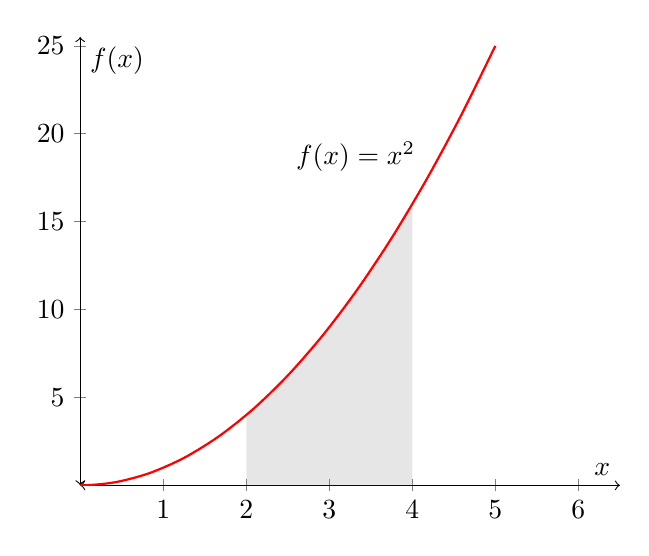
\begin{tikzpicture}
    \begin{axis}[
        xmin=0,xmax=6.5,
        ymin=0,ymax=25.5,
        axis x line=middle,
        axis y line=middle,
        axis line style=<->,
        xlabel={$x$},
        ylabel={$f(x)$}
        ]
    \addplot[red,thick,smooth,name path=A] {x^2} node [pos=.85,above left,color=black] {$f(x)=x^2$};
    \addplot[draw=none,name path=B] {0};
    \addplot[gray,opacity=.2] fill between[of=A and B,soft clip={domain=2:4}]; 
    \end{axis}
\end{tikzpicture}\bigskip

Area of two intersecting regions is given by $\int_{a}^{b}(f(x)-g(x))dx$.

\bigskip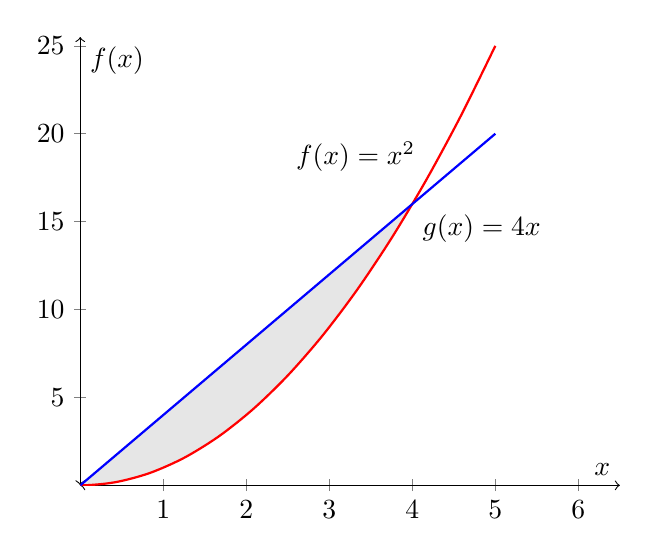
\begin{tikzpicture}
    \begin{axis}[
        xmin=0,xmax=6.5,
        ymin=0,ymax=25.5,
        axis x line=middle,
        axis y line=middle,
        axis line style=<->,
        xlabel={$x$},
        ylabel={$f(x)$}
        ]
    \addplot[red,thick,smooth,name path=A] {x^2} node [pos=.85,above left,color=black] {$f(x)=x^2$};
    \addplot[blue,thick,name path=B] {4*x} node [pos=.9,below right,color=black] {$g(x)=4x$};
    \addplot[gray,opacity=.2] fill between[of=A and B,soft clip={domain=0:4}]; 
    \end{axis}
\end{tikzpicture}\bigskip

Area of regions with multiple intersections is given by $\int_{a}^{b}|f(x)-g(x)|dx$, ignoring the central intersection point.

\bigskip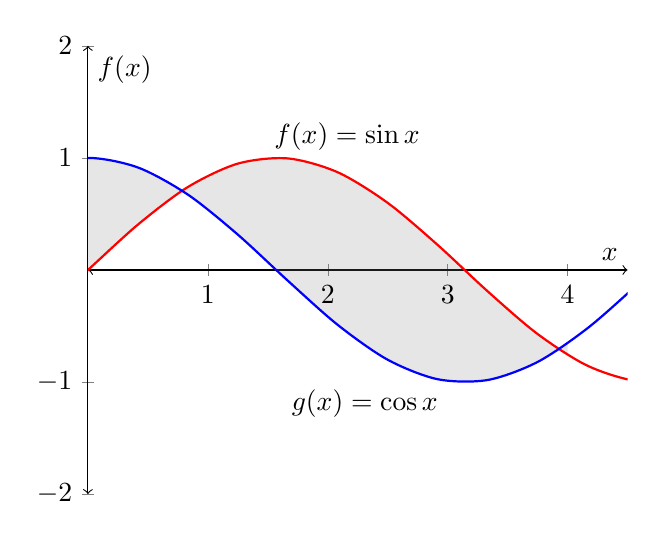
\begin{tikzpicture}
    \begin{axis}[
        xmin=0,xmax=4.5,
        ymin=-2,ymax=2,
        axis x line=middle,
        axis y line=middle,
        axis line style=<->,
        xlabel={$x$},
        ylabel={$f(x)$}
        ]
    \addplot[red,thick,smooth,name path=A] {sin(deg(x))} node [pos=.65,above right,color=black] {$f(x)=\sin{x}$};
    \addplot[blue,thick,smooth,name path=B] {cos(deg(x))} node [pos=.8,below left,color=black] {$g(x)=\cos{x}$};
    \addplot[gray,opacity=.2] fill between[of=A and B,soft clip={domain=0:4}]; 
    \end{axis}
\end{tikzpicture}\bigskip

$dy$ integration is similar to normal integration, but uses the $y$-axis for reference.
The following example uses $f(y)=sin(y)$ and $g(y)=cos(y)$, with the integral being $\int_{0}^{\pi/4}(g(y)-f(y))\:dy$.

\subsection{Volume around horizontal axes}\label{subsec:volume-around-horizontal-axes}

Given that $f(x)\geq{g(x)}\;\forall{x} \in [a,b]$, the integral is as follows for the region $R$ revolved around $x=0$.

\[V_x=\pi \int_{a}^{b}(f(x)^2-g(x)^2)\:dx\]

\bigskip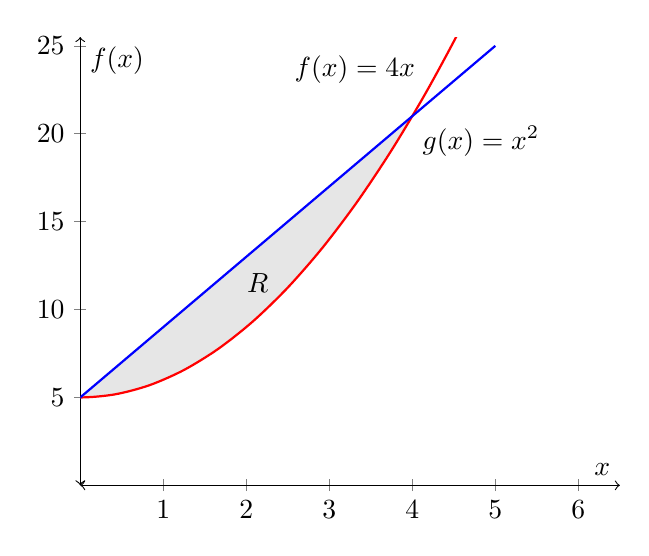
\begin{tikzpicture}
    \begin{axis}[
        xmin=0,xmax=6.5,
        ymin=0,ymax=25.5,
        axis x line=middle,
        axis y line=middle,
        axis line style=<->,
        xlabel={$x$},
        ylabel={$f(x)$}
        ]
    \addplot[red,thick,smooth,name path=A] {x^2+5} node [pos=.85,above left,color=black] {$f(x)=4x$};
    \addplot[blue,thick,name path=B] {4*x+5} node [pos=.9,below right,color=black] {$g(x)=x^2$};
    \addplot[gray,opacity=.2] fill between[of=A and B,soft clip={domain=0:4}]; 
    \node[label={180:{$R$}}] at (axis cs:2.5,11.5) {};
    \end{axis}
\end{tikzpicture}\bigskip

For the same region $R$ revolving around $x=2$, the radius of rotation (washer space) is reduced, so 2 is subtracted.
This would give the integral equation as the following.
If $x=-2$, for instance, 2 would be added as it increases the washer radius.

\[V_x=\pi \int_{0}^{4}((f(x)-2)^2-(g(x)-2)^2)\:dx\]

\bigskip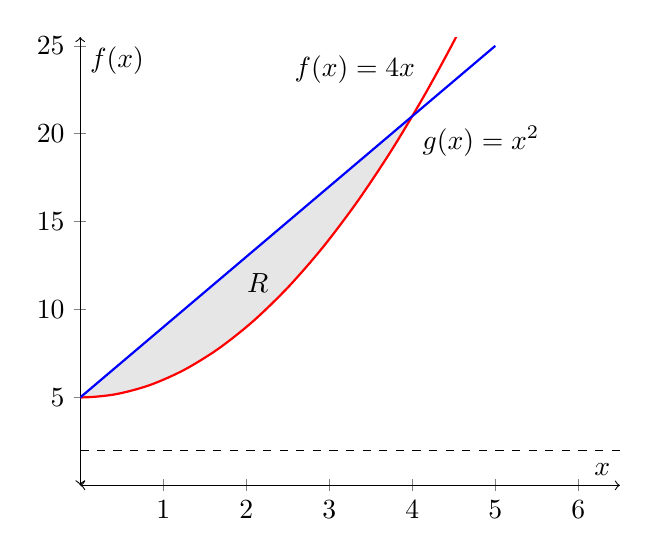
\begin{tikzpicture}
    \begin{axis}[
        xmin=0,xmax=6.5,
        ymin=0,ymax=25.5,
        axis x line=middle,
        axis y line=middle,
        axis line style=<->,
        xlabel={$x$},
        ylabel={$f(x)$}
        ]
    \addplot[red,thick,smooth,name path=A] {x^2+5} node [pos=.85,above left,color=black] {$f(x)=4x$};
    \addplot[blue,thick,name path=B] {4*x+5} node [pos=.9,below right,color=black] {$g(x)=x^2$};
    \addplot[gray,opacity=.2] fill between[of=A and B,soft clip={domain=0:4}]; 
    \node[label={180:{$R$}}] at (axis cs:2.5,11.5) {};
    \draw[dashed] (0,2) -- (7,2);
    \end{axis}
\end{tikzpicture}\bigskip

\subsection{Volume around vertical axes}\label{subsec:volume-around-vertical-axes}

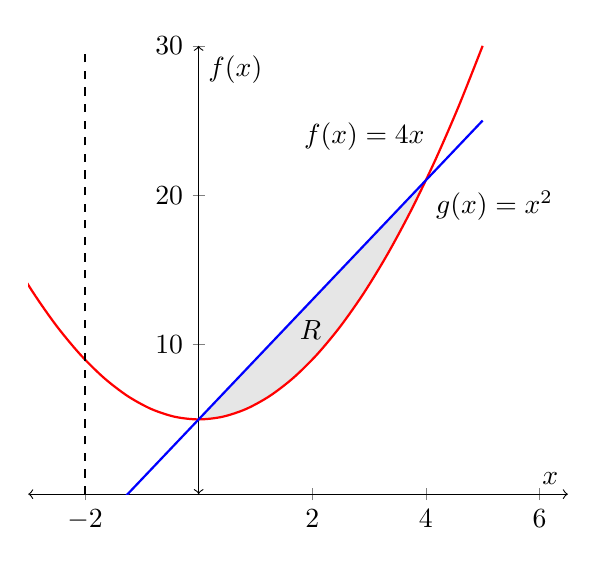
\begin{tikzpicture}
    \begin{axis}[
        xmin=-3,xmax=6.5,
        ymin=0,ymax=30,
        axis x line=middle,
        axis y line=middle,
        axis line style=<->,
        xlabel={$x$},
        ylabel={$f(x)$}
        ]
    \addplot[red,thick,smooth,name path=A] {x^2+5} node [pos=.85,above left,color=black] {$f(x)=4x$};
    \addplot[blue,thick,name path=B] {4*x+5} node [pos=.9,below right,color=black] {$g(x)=x^2$};
    \addplot[gray,opacity=.2] fill between[of=A and B,soft clip={domain=0:4}]; 
    \node[label={180:{$R$}}] at (axis cs:2.5,11) {};
    \draw[dashed] (-2,0) -- (-2,30);
    \end{axis}
\end{tikzpicture}\bigskip

Is given in the general form $V_y=2\pi \int_{a}^{b}(radius)(height)\:dx$.
The height is the value of $f(x)$ and the radius is some value of $x$ since this is with respect to the $y$-axis.
The preceding example is a rotation around $y=-2$, and the integral would be given by the following.

\[V_y=2\pi \int_{0}^{4}(x+2)(f(x)-g(x))\:dx\]

The procedure is the opposite when given a vertical axis on the other side of the graph in quadrant I, namely $x=7$.
This is because the radius would be given by $7-x$ since that difference is the distance between each varying point and $x=7$.
The formula would be the following.

\[V_y=2\pi \int_{0}^{4}(7-x)(f(x)-g(x))\:dx\]

\bigskip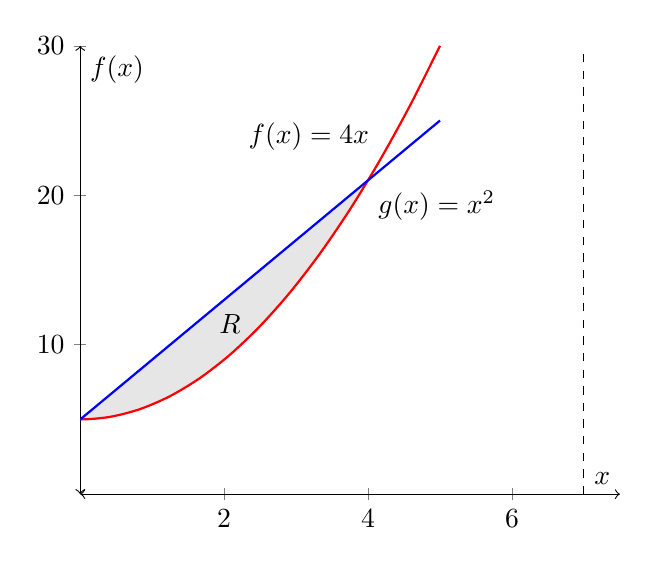
\begin{tikzpicture}
    \begin{axis}[
        xmin=0,xmax=7.5,
        ymin=0,ymax=30,
        axis x line=middle,
        axis y line=middle,
        axis line style=<->,
        xlabel={$x$},
        ylabel={$f(x)$}
        ]
    \addplot[red,thick,smooth,name path=A] {x^2+5} node [pos=.85,above left,color=black] {$f(x)=4x$};
    \addplot[blue,thick,name path=B] {4*x+5} node [pos=.9,below right,color=black] {$g(x)=x^2$};
    \addplot[gray,opacity=.2] fill between[of=A and B,soft clip={domain=0:4}]; 
    \node[label={180:{$R$}}] at (axis cs:2.5,11.4) {};
    \draw[dashed] (7,0) -- (7,30);
    \end{axis}
\end{tikzpicture}\bigskip

Notably, the last two examples can also be computed using $dy$ integration in a similar way to horizontal axis-based solids. 
However, the bottom function would become the top one and the limits would become the $y$-coordinates.
They are below.
Let $g(y)=\sqrt{y}$ and $f(y)=\frac{y}{4}$.

\begin{gather*}
    A_y=\pi \int_{5}^{21}((g(y)+2)^2-(f(y)+2)^2)dy\\
    A_y=\pi \int_{5}^{21}((7-g(y))^2-(7-f(y))^2)dy\\
\end{gather*}

\subsection{Volume with known cross-sections}

Let $s=f(x)-g(x)$ and $g(x)\leq{f(x)}\;\forall{x}\in{[a,b]}$.

\begin{itemize}
    \item Squares: $\int_{a}^{b}s^2dx$
    \item Rectangles (with the length being $n$ times the width): $\int_{a}^{b}ns^2dx$
    \item Equilateral triangles: $\int_{a}^{b}\frac{\sqrt{3}s^2}{4}dx$
    \item Semi-circles: $\int_{a}^{b}\frac{1}{8}\pi s^2dx$
    \item Right isosceles triangle: $\int_{a}^{b}\frac{1}{4}s^2dx$
\end{itemize}

\section{Infinite Series}\label{sec:infinite-series}
\subsection{Fundamental Series}

As listed below the harmonic series \ref{eq:1}, diverging due to P-series, and alternating series \ref{eq:2}, which converges according to AST.

\begin{equation}\label{eq:1}
    \sum_{n=1}^{\infty}\frac{1}{n}
\end{equation}
\begin{equation}\label{eq:2}
    \sum_{n=1}^{\infty}\frac{(-1)^n}{n}
\end{equation}

\subsection{P-series test}

A series in the form of $\sum_{n=1}^{\infty}\frac{1}{n^P}$.
If $P\leq{1}$, the series diverges, if $P>1$, it converges.

\subsection{n-th term test (divergence only)}

If $\lim_{n\to{\infty}}|a_n|\neq{0}$, the series diverges, else if it is 0, it is \textbf{inconclusive}.
But if a series diverges, \emph{it is not neccesarily due to the $n$-th term test}.

\subsection{Geometric series}

$\sum_{n=1}^{\infty}a_1r^{n-1}$ converges if and only if $|r|<1$.
A power series is a form of a geometric one.

\[\Rightarrow \sum_{n=1}^{\infty}a_1r^{n-1}=\frac{a_1}{1-r}\]

\subsection{Ratio test}

$\sum_{n=1}^{\infty}a_n$ converges if $\lim_{n\to{\infty}}|\frac{a_{n+1}}{a_n}|<1$.\\
$\sum_{n=1}^{\infty}a_n$ diverges if $\lim_{n\to{\infty}}|\frac{a_{n+1}}{a_n}|>1$.\\
The test if inconclusive is the result is 1.

\subsection{Alternating series test}

A decreasing alternating series, where $|a_{n+1}|<|a_n|$, converges if $\lim_{n\to{\infty}}a_n=0$.

\subsection{Taylor/Maclaurin Series}

\[\sum_{n=0}^{\infty}\frac{f^n(c)(x-c)^n}{n!}\]

Since the coefficient of each term is the $n$-th derivative, if given a term $T$, the derivative can be found by setting $\frac{f^n(c)(x-c)^n}{n!}=T$ in order to get an expression.

\bigskip A Maclaurin polynomial is a Taylor polynomial centered at $x=0$. Here are some common Maclaurin polynomial for function:
\begin{itemize}
    \item $\frac{1}{1-x}=1+x+x^2+x^3+\dots=\sum_{n=0}^{\infty}x^n$
    \item $e^x=1+\frac{x}{1!}+\frac{x^2}{2!}+\frac{x^3}{3!}+\dots=\sum_{n=0}^{\infty}\frac{x^n}{n!}$
    \item $\sin{x}=x-\frac{x^3}{3!}+\frac{x^5}{5!}-\frac{x^7}{7!}+\dots=\sum_{n=0}^{\infty}x^n$
    \item $\cos{x}=1-\frac{x^2}{2!}+\frac{x^4}{4!}-\frac{x^6}{6!}+\dots=\sum_{n=0}^{\infty}x^n$
    \item $\ln(1+x)=x-\frac{x^2}{2!}+\frac{x^3}{3!}-\frac{x^4}{4!}+\dots=\sum_{n=0}^{\infty}x^n$
\end{itemize}

\subsection{Trigonometric Identities}

Pythagorean Identities
\begin{itemize}
    \item $\sin^2{x}+\cos^2{x}=1$
    \item $\tan^2{x}+1=sec^2{x}$
    \item $1+\cot^2{x}=\csc^2{x}$
\end{itemize}\bigskip

Double-Angle Identities
\begin{itemize}
    \item $\sin{2x}=2\sin{x}\cos{x}$
    \item $\cos{2x}=\cos^2{x}-\sin^2{x}$
    \item $\tan{2x}=\frac{2\tan{x}}{1-\tan^2{x}}$
\end{itemize}

\end{document}